% ==================================================
% 4.6 計算效能、失敗案例與研究限制
% ==================================================
\section{計算效能、失敗案例與研究限制}
\label{sec:performance_failures_limits}

前述實驗分別呈現模型預測、導航與全身操作的結果，
其實際表現亦受到計算時間、命令承接與量測條件影響。
本節先以第 4.5 節的住宅代表案例分析計算耗時與控制期限，
再由相同整合紀錄集合整理未完成情形，
最後界定感知、接觸、幾何檢查及任務統計的適用範圍。
各項結果依對應的時間來源與評估條件解讀。

% ==================================================
% 4.6.1 求解時間與控制期限分析
% ==================================================
\subsection{求解時間與控制期限分析}
\label{subsec:solver_timing_deadline_analysis}

住宅案例的物理模擬、視覺推論、導航前端與控制工作程序同時執行。
計算耗時以主機時鐘量測，
並區分工作程序計算與派工至結果接收的來回時間：
\begin{equation}
    T_{\mathrm{rt}}
    =T_{\mathrm{in}}+T_{\mathrm{comp}}+T_{\mathrm{out}}.
    \label{eq:ch4_control_roundtrip_time}
\end{equation}
其中 $T_{\mathrm{in}}$ 包含輸入傳遞及等待工作程序開始的時間，
$T_{\mathrm{comp}}$ 為該次工作程序的計算時間，
$T_{\mathrm{out}}$ 為結果傳遞與接收時間。
工作程序另包含參考處理、最佳化、候選及停止軌跡核對等運算，
因此其耗時範圍大於單一 QP 數值求解。

\cref{tab:ch4_control_runtime}列出保存來回耗時的 $6688$ 筆回覆。
區段依控制模式劃分：初段包含導航與門把抓持，
穿門段亦包含其後導航，取放與回程段則涵蓋圓柱、抽屜及回程關門。
取放與回程資料中包含一筆正常結束回覆，
起動時未提供來回時間的紀錄則不納入此表。
開門段的來回耗時中位數為 $40.47$ ms，
第 $95$ 百分位數為 $57.85$ ms，
高於其餘三個區段的對應統計值。

\begin{table}[htbp]
    \centering
    \caption{住宅代表案例之控制計算與來回耗時（ms）}
    \label{tab:ch4_control_runtime}
    \begingroup
    \small
    \setlength{\tabcolsep}{4pt}
    \renewcommand{\arraystretch}{1.25}
    \begin{tabular}{l c c c c c}
        \hline
        控制區段 & 筆數
        & \shortstack{計算時間\\中位數}
        & \shortstack{來回時間\\中位數}
        & \shortstack{來回時間\\第 $95$ 百分位數}
        & \shortstack{來回時間\\最大值} \\
        \hline
        初段導航與抓持 & $360$  & $12.75$ & $13.23$ & $29.21$ & $38.16$ \\
        開門           & $189$  & $39.99$ & $40.47$ & $57.85$ & $60.15$ \\
        穿門及導航     & $1010$ & $16.38$ & $16.82$ & $31.02$ & $33.55$ \\
        取放與回程     & $5129$ & $23.57$ & $24.02$ & $37.97$ & $60.22$ \\
        \hline
    \end{tabular}
    \endgroup
\end{table}

\cref{fig:ch4_control_computation_timing}(a)呈現來回耗時的經驗累積分布。
以一倍速 $20$ Hz 所對應的 $50$ ms 主機週期作數值比較，
開門與取放回程段分別有 $28$ 與 $30$ 筆回覆超過此值。
本案例實際設定的外層來回預算為 $120$ ms，
且模擬依階段採用 $0.35$、$0.60$ 與 $0.70$ 的名目配速，
控制更新的 $50$ ms 為模擬時間步長。
上述回覆均未超過 $120$ ms，
結果仍須符合指定生效步與停止尾段條件才能承接。

\begin{figure}[htbp]
    \centering
    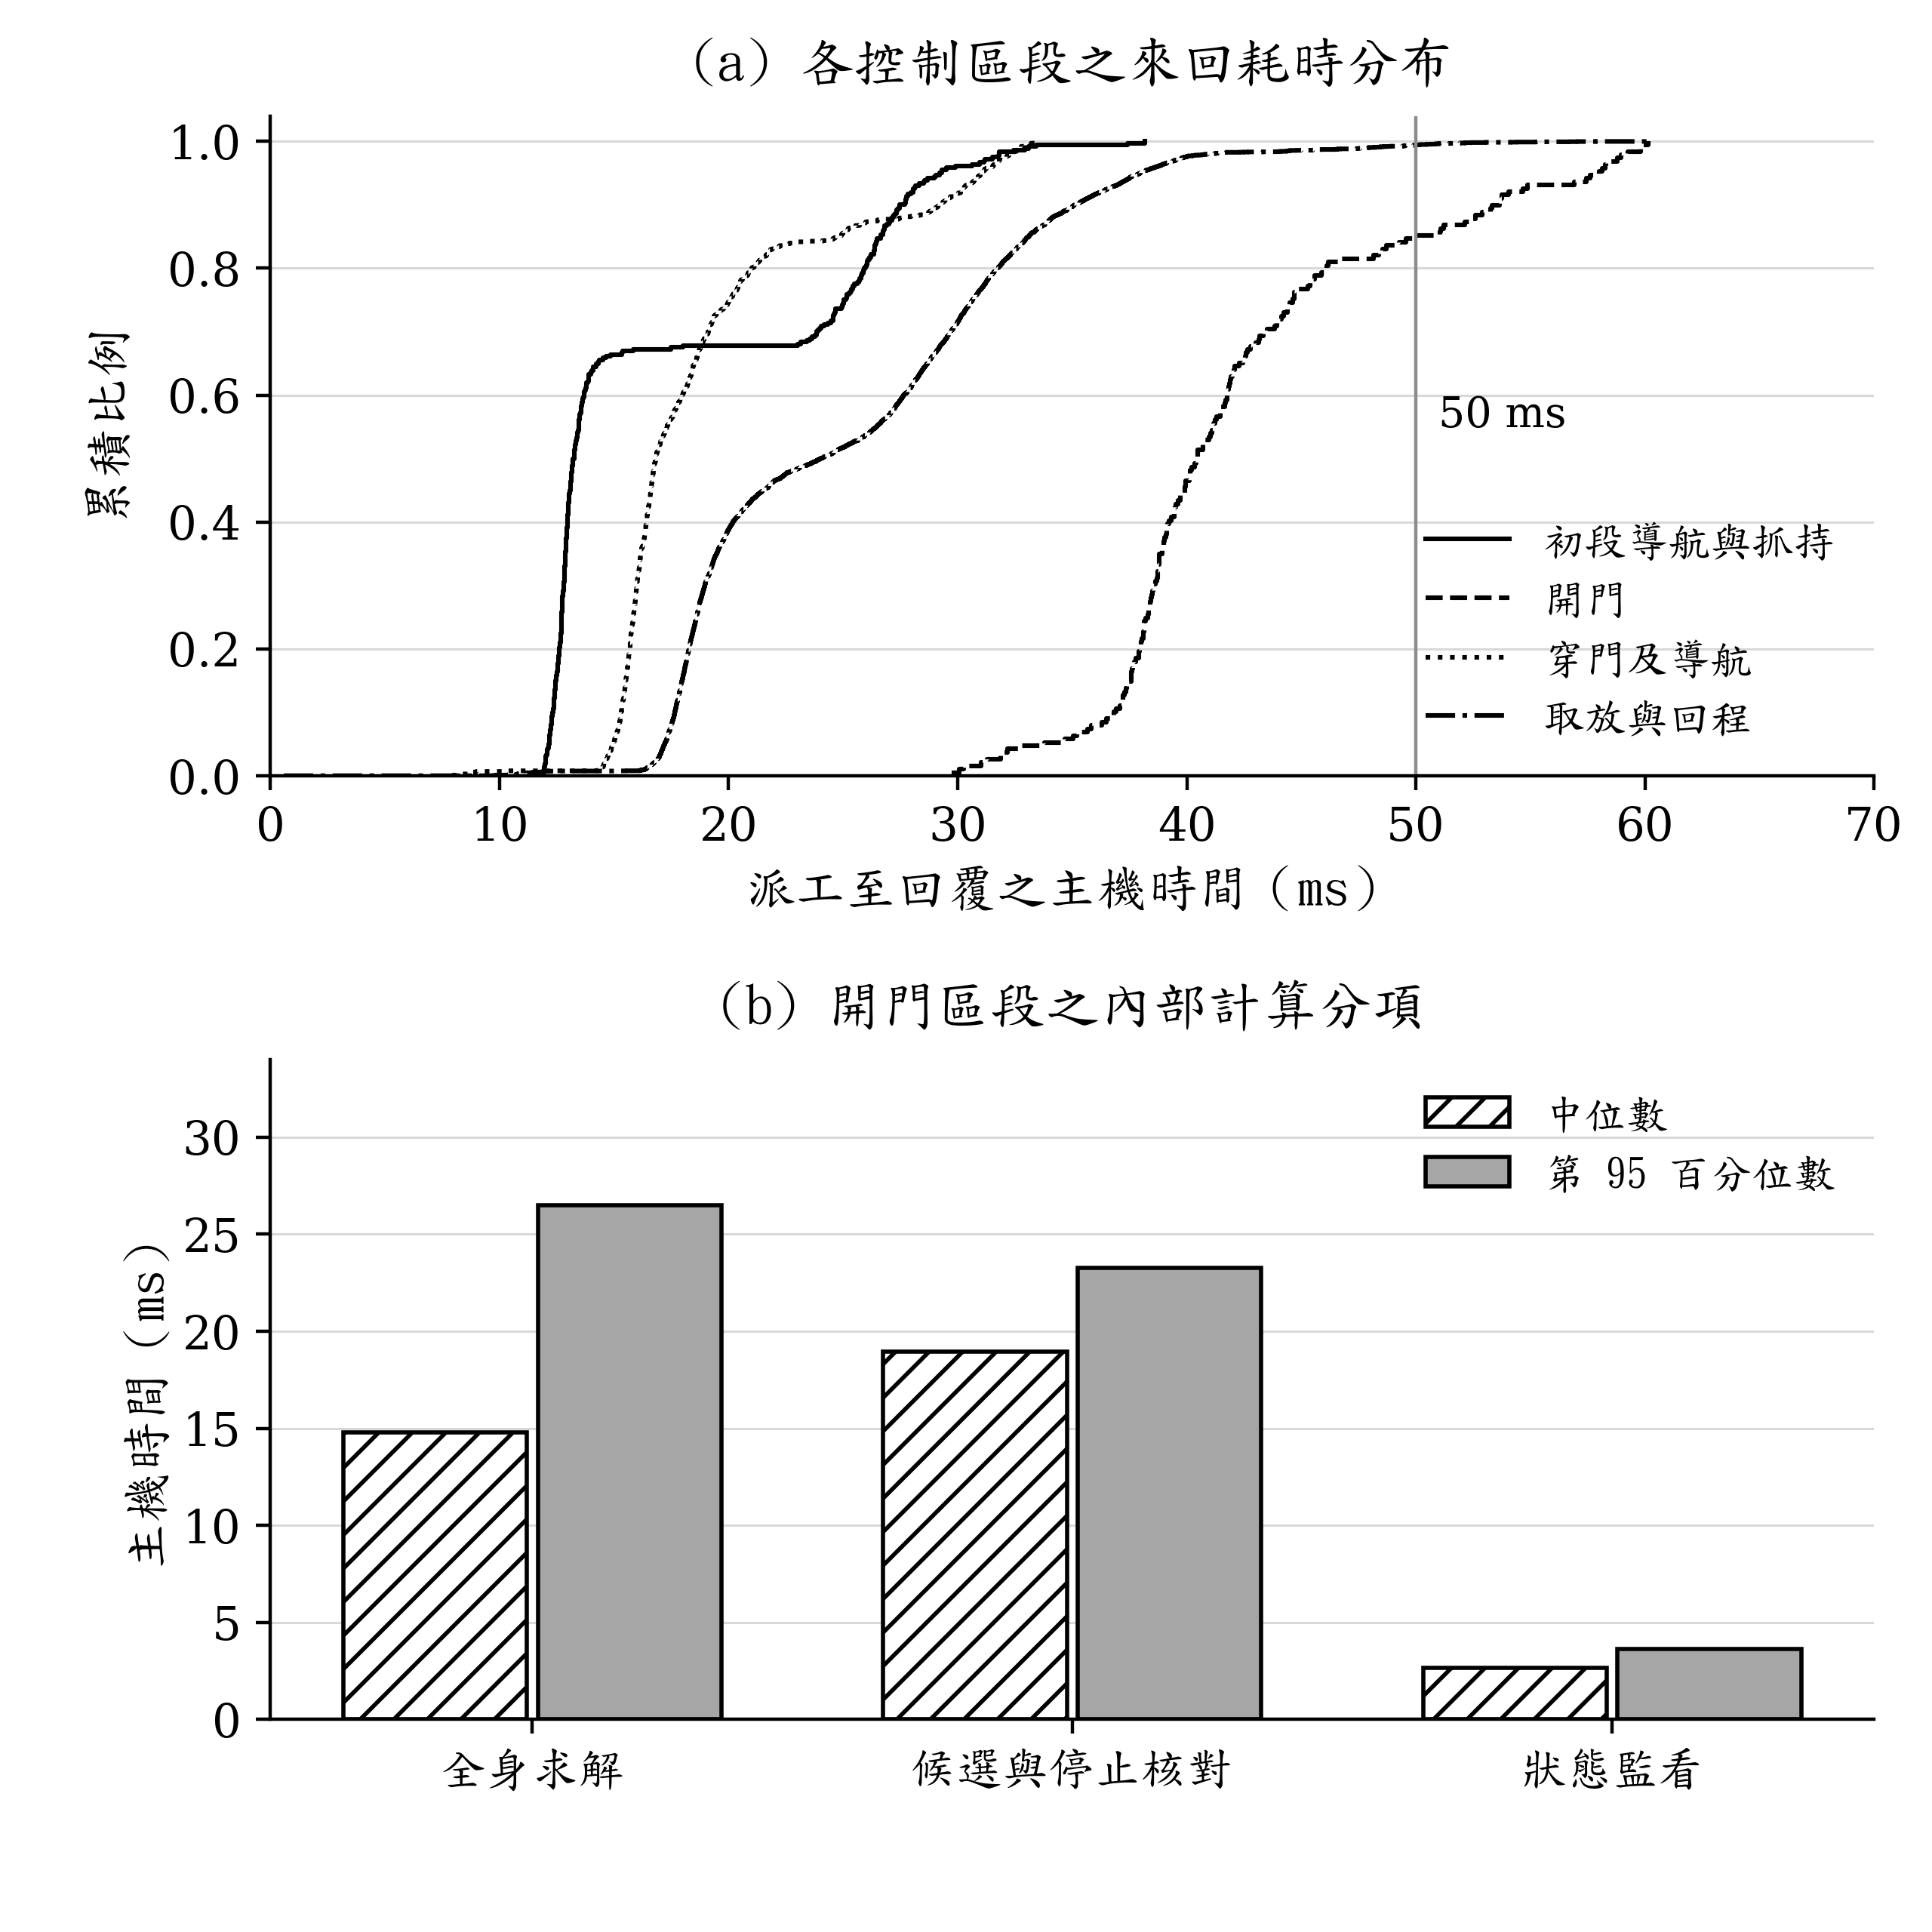
\includegraphics[width=0.98\textwidth]{figsrc/ch04/control_computation_timing.png}
    \caption{住宅代表案例之計算耗時：
    (a) 四個控制區段的來回耗時經驗累積分布，
    垂直線為一倍速 $20$ Hz 的 $50$ ms 主機週期對照；
    (b) 開門區段之全身求解、候選與停止核對及狀態監看耗時。
    各分項的中位數與第 $95$ 百分位數分別統計。}
    \label{fig:ch4_control_computation_timing}
\end{figure}

開門段的計算分項如\cref{fig:ch4_control_computation_timing}(b)所示。
全身求解、候選與停止核對及狀態監看的耗時中位數，
分別為 $14.80$、$18.95$ 與 $2.66$ ms。
在全身求解內部，矩陣組裝與 Goldfarb--Idnani 數值求解的中位數
分別約為 $8.39$ 與 $0.61$ ms。
這些分項具有包含關係，各項分位數亦分別計算，
用於辨識控制更新中主要的計算成本。
候選與停止核對需沿軌跡檢查構型與幾何條件，
其耗時在此案例中占有相當比例。

視覺處理另於背景程序執行。
保存的 $1853$ 筆分割耗時中，中位數為 $18.81$ ms，
第 $95$ 百分位數為 $24.66$ ms，最大值為 $368.24$ ms，出現在首筆紀錄。
感知更新頻率、資料年齡與控制更新頻率因此分別核對。
整段模擬器紀錄為 $371.56$ 模擬秒與 $606.0$ 主機秒，
平均實時因子約為 $0.613$，
其範圍與第 4.5 節由控制權交接事件起算的任務時間分開計算。
本組資料支持上述配速下的計算與執行結果，
一倍速連續 $20$ Hz 的控制期限仍需另行驗證。

% ==================================================
% 4.6.2 誤差來源與失敗案例分析
% ==================================================
\subsection{誤差來源與失敗案例分析}
\label{subsec:error_sources_failure_analysis}

第 4.5 節彙整的 $43$ 次紀錄中，共有 $14$ 次未完成完整住宅任務。
\cref{tab:ch4_residential_failure_categories}依各次保存的終止狀態分類，
每次紀錄僅計入一類。
此分類描述流程停止的位置及觸發條件，
個別根因仍需配合當時的狀態、輸入與幾何資料判斷。

\begin{table}[htbp]
    \centering
    \caption{住宅未完成紀錄之終止條件分類}
    \label{tab:ch4_residential_failure_categories}
    \begingroup
    \small
    \renewcommand{\arraystretch}{1.25}
    \begin{tabular}{p{0.37\textwidth} c p{0.43\textwidth}}
        \hline
        終止條件類別 & 次數 & 紀錄內容 \\
        \hline
        回覆未就緒或外層逾時 & $5$
        & 三次未於承接時取得回覆，兩次來回耗時超過預算 \\
        開門求解或內部預算中止 & $4$
        & 兩次求解失敗，兩次內部計算預算條件觸發 \\
        抽屜抓持與退出條件未達成 & $3$
        & 拉開時抓持條件失效、再次抓持逾時及退出距離不足各一次 \\
        接觸力保護中止 & $2$
        & 夾爪接觸力超過設定上限，物理模擬中止 \\
        \hline
        合計 & $14$ & \\
        \hline
    \end{tabular}
    \endgroup
\end{table}

計算相關案例顯示，外層來回時間與內部流程預算需分別處理。
兩次外層逾時的來回耗時為 $121.65$ 與 $140.60$ ms，
均超過當時的 $120$ ms 預算。
另兩次開門流程在內部耗時約 $95.1$ ms 時觸發預算條件，
其外層來回時間約為 $97$ ms，仍未取得可繼續承接的候選。
因此，單看平均耗時或外層上限，無法涵蓋所有控制段的接受條件。

操作相關案例則反映到位、抓持及退出各有獨立條件。
再次接近抽屜把手的一次紀錄中，
確認階段的雙指接觸力皆為零，最後因抓持證據逾時而停止。
另一次退出時，末端反向位移僅約 $31.5$ mm，
未達所需的 $90$ mm，故未接續後續任務。
兩次接觸力保護紀錄的峰值分別約為 $41.99$ 與 $49.18$ N，
超過設定的 $40$ N 上限。
該兩例中止後未繼續物理步進，保留當時狀態，
其後的減速與停穩過程沒有量測證據。

其餘 $12$ 次未完成紀錄曾進入停止尾段。
停穩核對要求最終命令歸零、在途輸入排清，
並連續 $0.3$ s 符合
\begin{equation}
    \|v_B\|_2<0.003\ \mathrm{m/s},\qquad
    |\omega_B|<0.003\ \mathrm{rad/s},\qquad
    \|\dot q_a\|_\infty<0.002\ \mathrm{rad/s}.
    \label{eq:ch4_measured_stopping_conditions}
\end{equation}
判定期限為最後非零輸入後的 $4$ s。
其中 $10$ 例在 $0.37$--$1.78$ s 內取得符合條件的連續區間，
另外兩例在保存的觀測期間未通過。

\cref{fig:ch4_stopping_residual_counterexamples}呈現兩個未通過案例的逐軸最大關節速率。
抽屜拉開中止與開門回覆逾時後，
最後一筆量測的最大關節速率分別約為 $5.10$ 與 $2.28$ mrad/s，
且未形成所需的連續低速區間。
停止尾段播放完成與實際機器人停穩因此分別核對，
接觸耦合、關節追蹤及殘餘運動仍是後續驗證的重要項目。

\begin{figure}[htbp]
    \centering
    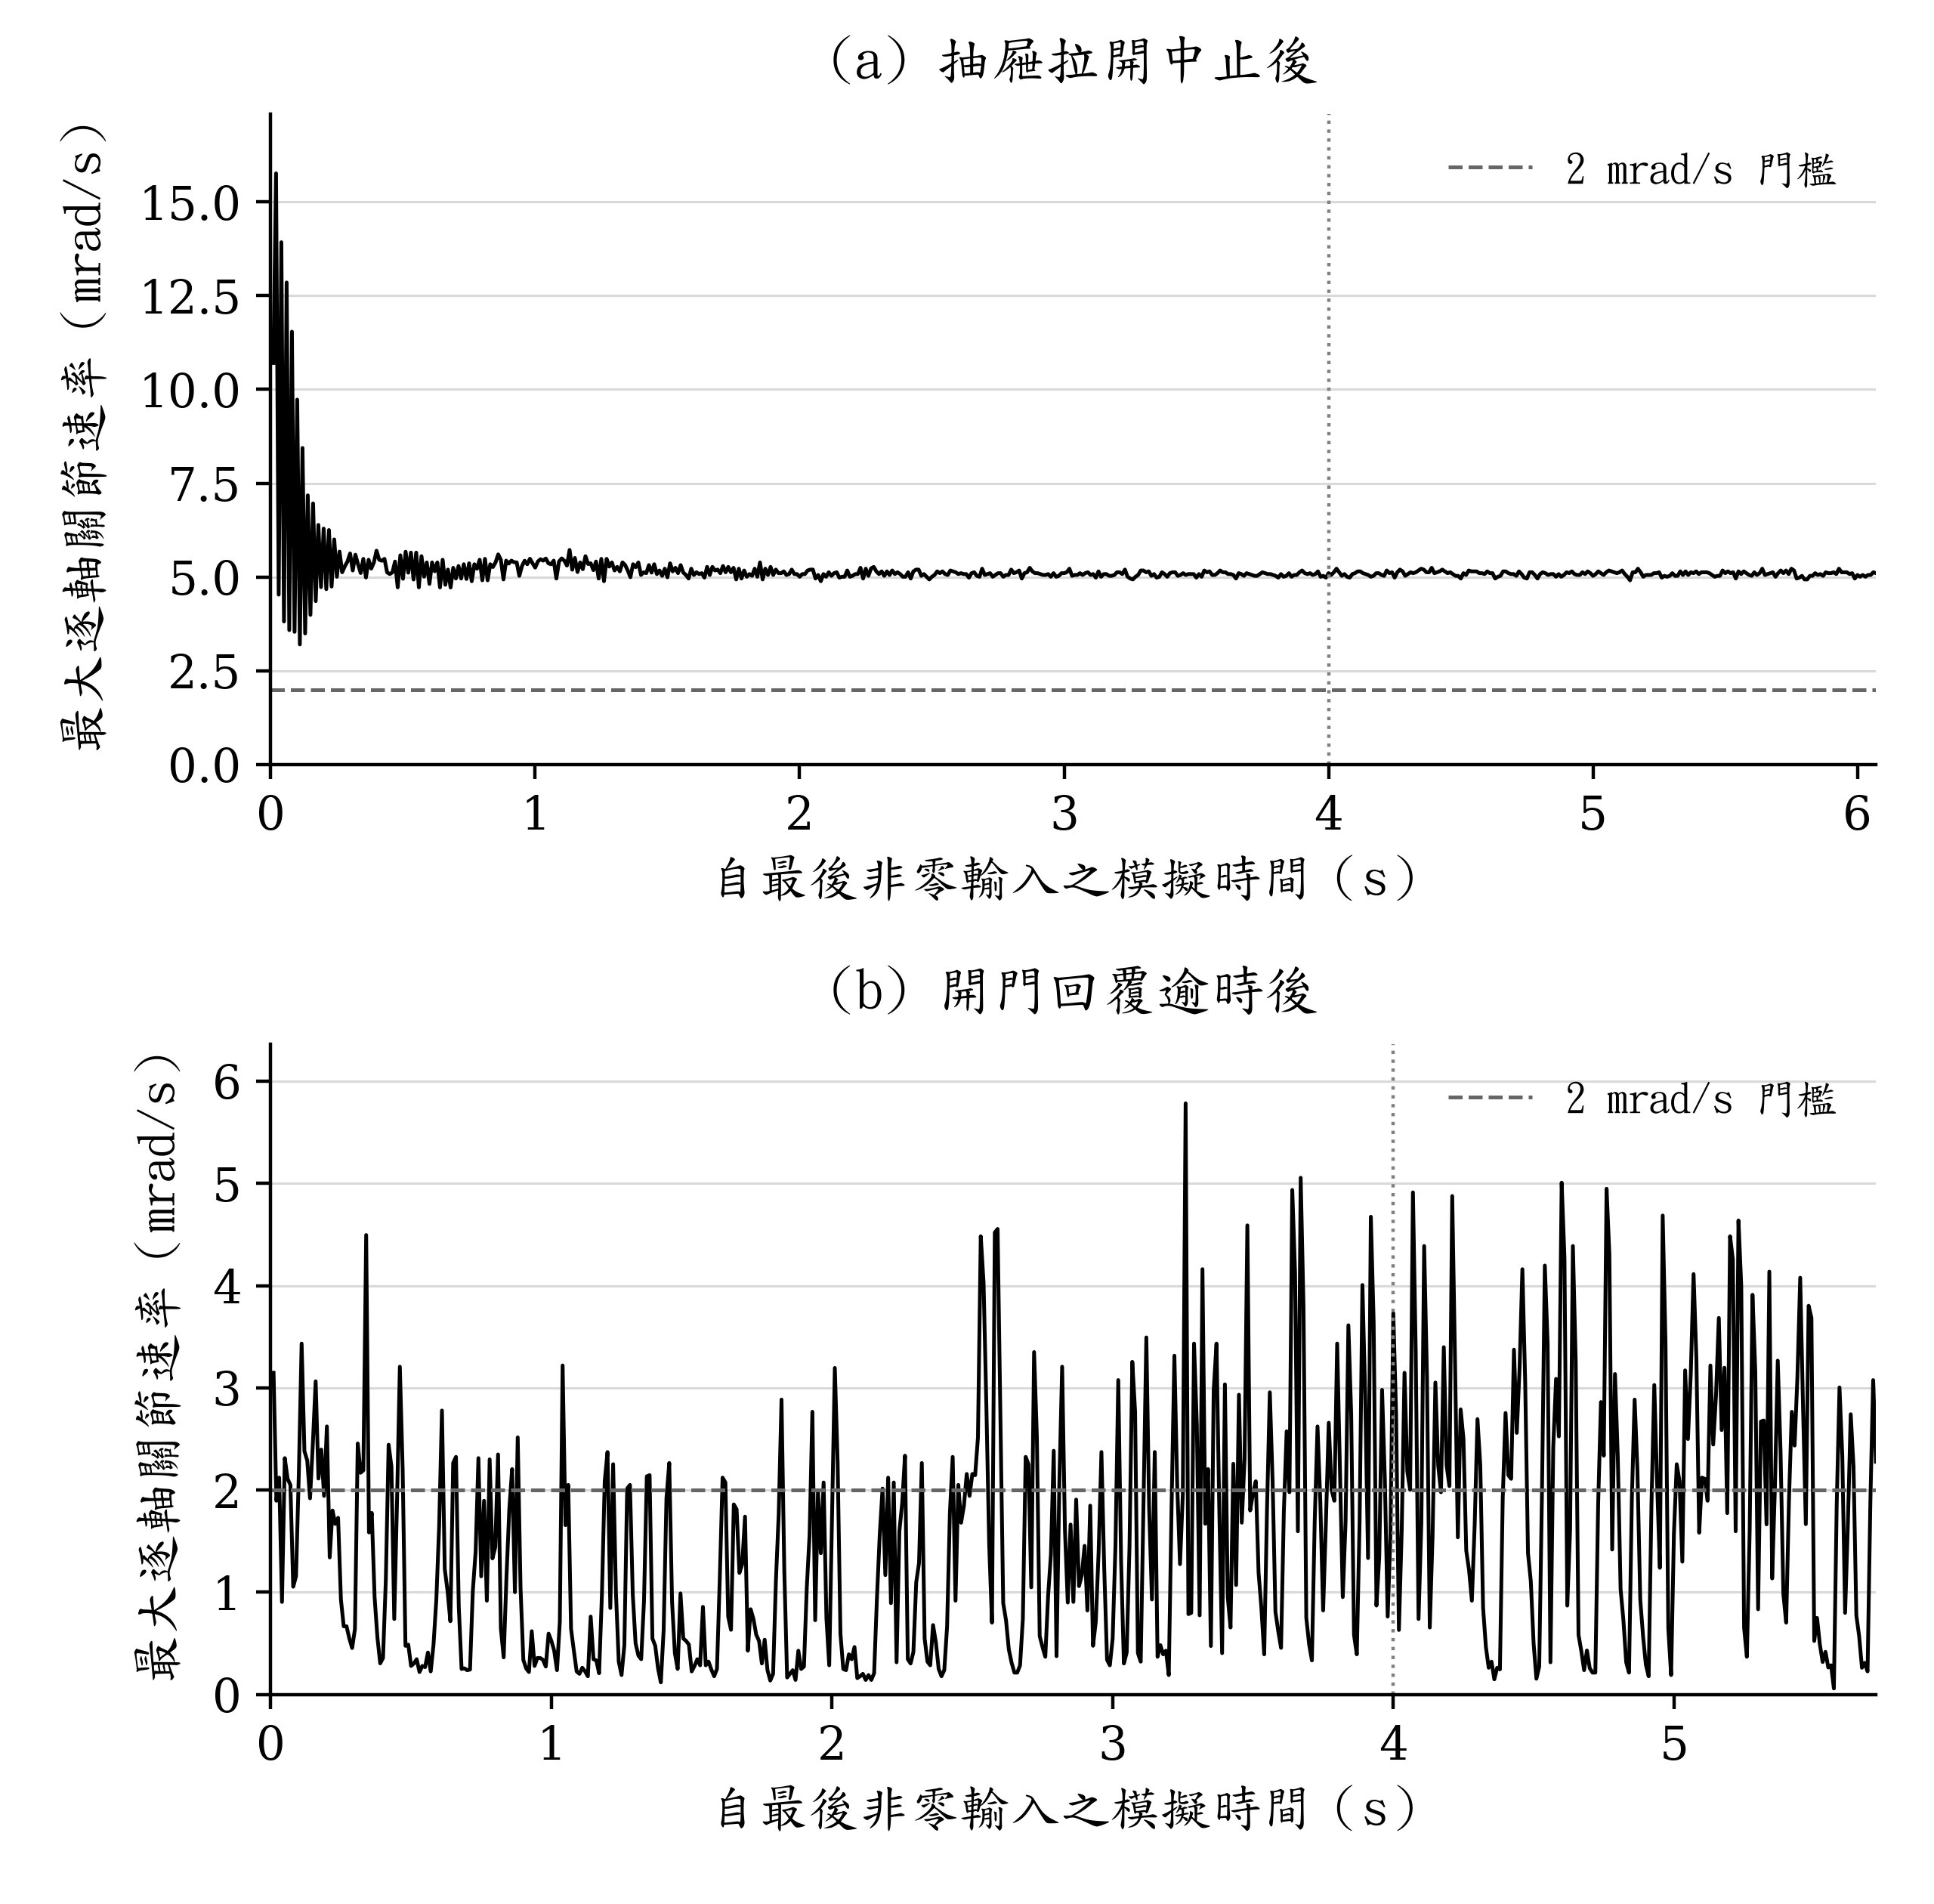
\includegraphics[width=0.98\textwidth]{figsrc/ch04/stopping_residual_counterexamples.png}
    \caption{停止尾段後未通過停穩判定的兩個案例：
    (a) 抽屜拉開中止後；(b) 開門回覆逾時後。
    曲線為每一物理步由關節位置差分取得的最大逐軸速率；
    水平虛線為 $2$ mrad/s 門檻，垂直點線為 $4$ s 判定期限。
    完整停穩條件另包含底盤速率、命令歸零及連續保持時間。}
    \label{fig:ch4_stopping_residual_counterexamples}
\end{figure}

% ==================================================
% 4.6.3 方法適用範圍與限制
% ==================================================
\subsection{方法適用範圍與限制}
\label{subsec:method_scope_limitations}

本研究的主要證據來自指定模擬場景與已配置的操作目標，
各項比較的範圍如\cref{tab:ch4_evidence_scope_limits}所示。
模型辨識與離線重播支持位置介面的預測描述，
導航與操作結果則呈現相應配置下的控制表現。
不同平台、控制版本與時間定義依前述各節分別保留。
第 4.2 節的偏置更新採固定軌跡離線重播評估；
線上偏置與末端積分補償的個別貢獻，
仍需於相同初始條件下進行獨立消融。

\begin{table}[htbp]
    \centering
    \caption{實驗證據之適用範圍與限制}
    \label{tab:ch4_evidence_scope_limits}
    \begingroup
    \small
    \renewcommand{\arraystretch}{1.25}
    \begin{tabular}{p{0.17\textwidth} p{0.35\textwidth} p{0.36\textwidth}}
        \hline
        評估面向 & 目前證據 & 適用範圍與限制 \\
        \hline
        執行模型
        & 設定點追蹤辨識、單步及多步離線重播
        & 對應辨識增益與資料條件；負載及控制介面改變時需重新驗證 \\
        導航避障
        & 共同路線到達、平面淨空與模組消融
        & 受外形近似、感測與場景規則影響；幾何重疊與實際接觸分別解讀 \\
        全身操作
        & 底盤與末端協同、抽屜與住宅任務銜接
        & 持物採固定相對位姿假設，尚未涵蓋完整摩擦抓持與滑移 \\
        視覺感知
        & 模擬 RGB-D 目標估測與時間對齊
        & 物件尺寸與家具幾何具有先驗，實體影像與感測誤差尚需驗證 \\
        計算執行
        & 設定配速下的計算耗時與停止紀錄
        & 使用分階段配速與 $120$ ms 外層預算，尚未完成一倍速控制期限驗證 \\
        任務統計
        & 配對案例與整合紀錄之完成及中止情形
        & 部分資料包含版本修正，條件時間比較限於完成案例 \\
        \hline
    \end{tabular}
    \endgroup
\end{table}

感知與定位方面，住宅模擬以物理位姿提供底盤里程，
雷射由無額外雜訊的射線量測建立，
相機轉換使用渲染時刻的機器人構型。
目前結果尚未包含實體定位漂移、相機標定誤差與影像域差異的共同影響。
物件搜尋區域、尺寸與家具機構亦具有先驗，
因此觀測導引的結果限於這些先驗與有效量測所涵蓋的範圍。

接觸與幾何方面，固定相對位姿能維持持物及閉鏈操作的運動學關係，
但摩擦不足、滑移與柔順接觸需另行建模及驗證。
筆狀物件使用粗筆代理模型，其抓取條件與細筆不同。
線上幾何核對涵蓋已啟用的機器人、家具與盒體近似，
持物外形及盒內既有物件尚未完整納入碰撞預測。
CBF 的局部線性化、鬆弛與有限步取樣，
也使實驗淨空結果限於所使用的幾何與離散檢查條件。

命令一致性方面，住宅代表案例保存了最終放行值與執行回授，
其提案對放行的檢查另記錄 $219$ 筆未配對提示及 $41$ 筆差異提示。
當時配置沿用實際放行值進行預測與執行，
上述提示以紀錄方式保留，並未全部作為中止條件。
因此，流程完成仍需配合完整的最終輸入重播，
才能進一步核對全程預測與執行的一致性。

後續驗證需先固定控制與任務配置，
補齊放行命令、停止尾段與實際運動之間的逐步對應，
再增加感測擾動、接觸條件與重複測試。
第五章依本章證據整理研究貢獻，
並提出計算期限、實體抓持與動態場景驗證的後續工作。
